\documentclass[11pt]{article}
\usepackage[margin=1in]{geometry}
\usepackage{amsmath,amssymb,graphicx,microtype,booktabs}
\usepackage[font=small,skip=3pt]{caption}
\usepackage[hidelinks]{hyperref}
\usepackage{enumitem}
\setlist{nosep,leftmargin=1.2em}
\setlength{\parindent}{0pt}
\setlength{\parskip}{2.5pt plus 1pt minus 1pt}
\setlength{\textfloatsep}{5pt plus 2pt minus 2pt}
\setlength{\intextsep}{7pt plus 2pt minus 2pt}
\title{\vspace{-1.6em}\textbf{Nearby Examples, New Proofs}\vspace{-0.5em}}
\author{J. R. Landers\\[-1pt]\small Retrieval-guided generation in LeanDojo Benchmark 4}
\date{\vspace{-1.2em}}

\begin{document}
\maketitle
\vspace{-1.6em}

When a model proposes a formal proof, resemblance is not enough.  Lean elaborates the script
into a proof term, and its small trusted kernel either accepts that term or rejects it.  This gives
an unusually sharp experimental outcome: a generated argument is not graded for plausibility but
checked for correctness in the theorem's original mathematical environment.

Retrieval offers a simple intervention.  Before asking for a proof, show the model several proved
theorems that resemble the target.  The examples may supply a premise, a useful tactic, or the shape
of an argument.  They may also distract.  The practical question is therefore not whether theorem
statements have neighborhoods, but whether the right neighborhoods help produce new proofs.

Two earlier studies separated proof procedure from mathematical subject and then recovered the same
distinction in learned embeddings \cite{textures,geometry}.  The second also found a local bridge:
nearby statement vectors had more-similar recorded proof traces than a matched random baseline.
The present experiment crosses that bridge.  On 100 held-out Lean theorems, semantically retrieved
examples yield the best observed proof rate: 24 theorems solved in three attempts, against 21 for
lexical retrieval, 16 with no examples, and 14 with random examples.

\paragraph{Four kinds of context.}
Let $Q=\{1,\ldots,m\}$ index the $m=100$ target theorems and let $T$ be a bank of
$N=9{,}637$ training theorems.  Target $i\in Q$ has statement $s_i$; training record
$j\in T$ has statement $s_j$ and its complete source declaration, including the recorded proof.
Training and test splits follow LeanDojo \cite{leandojo}; retrieval never uses a test-split proof.
Exact statement duplicates and candidates with cosine
similarity above $0.98$ are removed before examples are selected.

For the semantic condition, let $x_i,x_j\in\mathbb{R}^{1024}$ be the statement embeddings and
rank training record $j$ by
\[
 \operatorname{cos}(i,j)=
 \frac{x_i\mathbin{\cdot}x_j}{\lVert x_i\rVert_2\lVert x_j\rVert_2},
 \qquad
 \lVert x\rVert_2=\left(\sum_{r=1}^{1024}x_r^2\right)^{1/2}.
\]
Here $x_i\mathbin{\cdot}x_j$ is the usual dot product and $\lVert x\rVert_2$ is Euclidean length.
The four largest eligible cosine scores supply the examples.

BM25 supplies a lexical comparison.  Let $q_i$ be the set of tokens in target statement $s_i$,
$f_{jw}$ the number of occurrences of token $w$ in training statement $s_j$, $\ell_j$ its token
length, $\bar\ell$ the mean training-statement length, and $n_w$ the number of training statements
containing $w$.  With $k_1=1.5$ and $b=0.75$, its score is
\[
 B(i,j)=\sum_{w\in q_i}
 \log\!\left(1+\frac{N-n_w+\tfrac12}{n_w+\tfrac12}\right)
 \frac{f_{jw}(k_1+1)}
 {f_{jw}+k_1(1-b+b\ell_j/\bar\ell)}.
\]
The logarithmic factor emphasizes rare tokens; the denominator discounts repetition and adjusts
for document length \cite{bm25}.  The remaining conditions show four uniformly random eligible
training declarations or no examples at all.  Thus semantic and BM25 retrieval differ in how they
define relevance, while random retrieval controls for merely adding demonstrations.

\paragraph{Generation and proof checking.}
Let $C=\{0,R,B,S\}$ denote no retrieval, random, BM25, and semantic retrieval.  Claude Sonnet 4.5
receives one frozen prompt for target $i$ and condition $c\in C$, then produces three stochastic
candidates indexed by $a\in\{1,2,3\}$.  Temperature is $0.4$ and output is capped at 500 tokens.
For each candidate define
\[
 Y_{ica}=\begin{cases}
 1,&\text{if Lean accepts candidate $a$ in the original source context},\\
 0,&\text{otherwise},
 \end{cases}
 \qquad
 P_i^{(c,k)}=\max_{1\leq a\leq k}Y_{ica},
\]
\[
 \widehat p_c(k)=\frac1m\sum_{i=1}^m P_i^{(c,k)}.
\]
Thus $P_i^{(c,k)}$ says whether condition $c$ solves target $i$ within its first $k$ candidates,
and $\widehat p_c(k)$ is the empirical pass@$k$ rate.  All 1,200 candidates are checked at Mathlib
commit \texttt{3c307701} with Lean 4.6.0-rc1.  The theorem being proved is replaced in its source
file, so a candidate cannot succeed by importing or citing the existing declaration.

\begin{figure}[t]
  \centering
  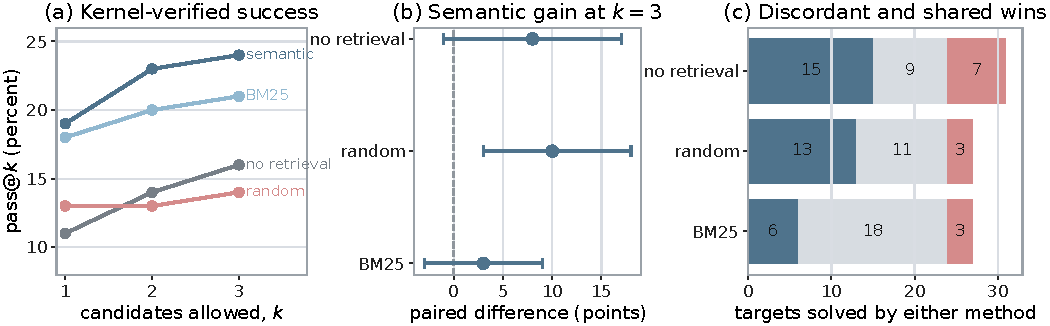
\includegraphics[width=\textwidth]{retrieval_generation_results.pdf}
  \caption{Kernel-verified proof generation on the same 100 targets.  (a) Semantic retrieval has
  the highest pass rate for one, two, and three candidates.  (b) Semantic-minus-baseline pass@3
  differences with 95\% paired target-bootstrap intervals.  (c) Among targets solved by either
  method, blue, gray, and red segments respectively show semantic-only, shared, and baseline-only
  successes.}
  \label{fig:retrieval}
\end{figure}

\paragraph{What retrieval changed.}
The complete outcomes are
\[
\begin{array}{lrrrr}
\toprule
\text{condition} & \text{pass@1} & \text{pass@2} & \text{pass@3} & \text{accepted candidates}\\
\midrule
\text{no retrieval} & 11\% & 14\% & 16\% & 38/300\\
\text{random}       & 13\% & 13\% & 14\% & 33/300\\
\text{BM25}         & 18\% & 20\% & 21\% & 52/300\\
\text{semantic}     & \mathbf{19\%} & \mathbf{23\%} & \mathbf{24\%} & \mathbf{61/300}\\
\bottomrule
\end{array}
\]
Random demonstrations do not help: their pass@3 rate is slightly below the theorem-only prompt.
Relevant examples do help in point estimate.  Semantic retrieval gains eight percentage points over
no retrieval and ten over random retrieval; BM25 gains five and seven points respectively.

Because every condition uses the same targets, paired rather than independent uncertainty is
appropriate.  For baseline $b\in\{0,R,B\}$, define the targetwise difference
$D_i^{(b)}=P_i^{(S,3)}-P_i^{(b,3)}\in\{-1,0,1\}$ and its mean
$\widehat\Delta_b=m^{-1}\sum_iD_i^{(b)}$.  The intervals in Figure~\ref{fig:retrieval}(b)
resample the $m$ target indices with replacement 10,000 times and take the 2.5th and 97.5th
percentiles of the resulting $\widehat\Delta_b$ values.

An exact McNemar comparison uses only discordant targets.  Let $n_+$ count targets solved by
semantic retrieval but not baseline $b$, and $n_-$ the reverse.  Under equal paired success
probability, $n_+$ conditional on $n_++n_-$ has a binomial distribution with success probability
$1/2$.  Semantic versus random has $(n_+,n_-)=(13,3)$, difference $+10$ points, bootstrap interval
$[3,18]$ points, and two-sided exact $p=0.021$.  Against no retrieval the corresponding values are
$(15,7)$, $+8$, $[-1,17]$, and $p=0.134$; against BM25 they are $(6,3)$, $+3$, $[-3,9]$, and
$p=0.508$.  These unadjusted pilot comparisons are descriptive: only the random baseline is clearly
separated at this sample size.

\paragraph{What the comparison says.}
The experiment supports a useful but bounded claim.  Showing proofs of related statements improves
generation, and semantic neighborhoods carry operational information beyond the mere presence of
examples.  The geometry is doing work.  It is not yet doing demonstrably more work than lexical
retrieval.  Semantic and BM25 prompts share only 1.27 of four examples on average, and share none
for 24 targets, yet their success sets overlap heavily: 18 targets are solved by both, six only by
semantic retrieval, and three only by BM25.

Random examples also reveal a cost of irrelevant context.  They produce the most output tokens and
38 truncated responses, compared with 17 under semantic retrieval; none of the 83 truncated
responses across all conditions pass.  Among other rejections, Lean reports unknown identifiers,
unsolved goals, tactic failures, and elaboration errors.  One unusually expensive theorem times out
in all 12 of its checks.  Removing it leaves 99 paired targets and the same success counts, so the
ordering is unchanged.

The 1,200 model calls use 817,170 input tokens and 131,471 output tokens.  Observed inference cost is
\$4.42; a conservative reserve for six responses lost to a command-line encoding failure raises the
accounted total to \$4.56.  Generation takes 22.7 minutes and eight-worker local kernel checking
takes 72.5 minutes after setup.  Exact prompts, responses, token counts, source contexts, verifier
outputs, hashes, and analysis code are retained.

\paragraph{What remains open.}
This is one model, one prompt, one temperature, one library snapshot, and 100 targets.  The model API
exposes no sampling seed, proof declarations vary in length, and a 500-token cap may suppress longer
arguments.  Pass@3 measures whether retrieval helps this generator under this budget, not whether
the retrieved proof is mathematically the same argument.  A larger paired study should emphasize
semantic versus BM25 retrieval, preclassify slow source files, and freeze any higher output limit
before generation.

The three notes now trace a progression: proof style and mathematical subject form different global
structures; statement and proof embeddings retain that distinction while sharing local
neighborhoods; and those neighborhoods can help a model construct kernel-accepted proofs.  The last
step is practical rather than metaphysical.  Similarity does not prove a theorem, but it can put a
useful proof within reach.

\begin{thebibliography}{9}\scriptsize
\setlength{\itemsep}{0pt}
\bibitem{textures} J. R. Landers. ``Textures of Modern Formal Mathematics.'' Remarks on LeanDojo Benchmark 4, 2026.
\bibitem{geometry} J. R. Landers. ``What Statements Know, What Proofs Do.'' Semantic views of LeanDojo Benchmark 4, 2026.
\bibitem{leandojo} K. Yang et al. ``LeanDojo: Theorem Proving with Retrieval-Augmented Language Models.'' NeurIPS Datasets and Benchmarks, 2023.
\bibitem{bm25} S. Robertson and H. Zaragoza. ``The Probabilistic Relevance Framework: BM25 and Beyond.'' Foundations and Trends in Information Retrieval 3(4), pp. 333--389, 2009.
\end{thebibliography}

\end{document}
